%%%%%%%%%%%%%%%%%%%%%%%%%%%%%%%%%%%%%%%%%
% Beamer Presentation
% LaTeX Template
%
% This template has been downloaded from:
% http://www.LaTeXTemplates.com
%
% This template has been altered after it was downloaded from the 
% above link
%
% License:
% CC BY-NC-SA 3.0 (http://creativecommons.org/licenses/by-nc-sa/3.0/)
%
%%%%%%%%%%%%%%%%%%%%%%%%%%%%%%%%%%%%%%%%%

%----------------------------------------------------------------------------------------
%	PACKAGES AND THEMES


\documentclass{beamer}

\mode<presentation> {

% The Beamer class comes with a number of default slide themes
% which change the colors and layouts of slides. Below this is a list
% of all the themes, uncomment each in turn to see what they look like.

%\usetheme{default}
%\usetheme{AnnArbor}
%\usetheme{Antibes}
%\usetheme{Bergen}
%\usetheme{Berkeley}
%\usetheme{Berlin}
%\usetheme{Boadilla}
%\usetheme{CambridgeUS}
%\usetheme{Copenhagen}
%\usetheme{Darmstadt}
%\usetheme{Dresden}
\usetheme{Frankfurt}
%\usetheme{Goettingen}
%\usetheme{Hannover}
%\usetheme{Ilmenau}
%\usetheme{JuanLesPins}
%\usetheme{Luebeck}
%\usetheme{Madrid}
%\usetheme{Malmoe}
%\usetheme{Marburg}
%\usetheme{Montpellier}
%\usetheme{PaloAlto}
%\usetheme{Pittsburgh}
%\usetheme{Rochester}
%\usetheme{Singapore}
%\usetheme{Szeged}
%\usetheme{Warsaw}

% As well as themes, the Beamer class has a number of color themes
% for any slide theme. Uncomment each of these in turn to see how it
% changes the colors of your current slide theme.

%\usecolortheme{albatross}
%\usecolortheme{beaver}
%\usecolortheme{beetle}
%\usecolortheme{crane}
%\usecolortheme{dolphin}
\usecolortheme{dove}
%\usecolortheme{fly}
%\usecolortheme{lily}
%\usecolortheme{orchid}
%\usecolortheme{rose}
%\usecolortheme{seagull}
%\usecolortheme{seahorse}
%\usecolortheme{whale}
%\usecolortheme{wolverine}

% Here is an overview of possible theme and colortheme combinations:
% https://hartwork.org/beamer-theme-matrix/

%\setbeamertemplate{footline} % To remove the footer line in all slides uncomment this line
%\setbeamertemplate{footline}[page number] % To replace the footer line in all slides with a simple slide count uncomment this line

%\setbeamertemplate{navigation symbols}{} % To remove the navigation symbols from the bottom of all slides uncomment this line
}

\usepackage{graphicx} % Allows including images
\usepackage{booktabs} % Allows the use of \toprule, \midrule and \bottomrule in tables
\usepackage{appendixnumberbeamer} % Allows use of \appendix. Slides appearing after will not be part of the frame counter or navigation panel
\usepackage{todonotes} % Allows use of \missingfigure

% Following lines makes a section overview at the beginning of each section 
\setbeamertemplate{caption}{\raggedright\insertcaption\par}
\AtBeginSection[]
{
 \begin{frame}<beamer>
 %\frametitle{Plan}
 \tableofcontents[currentsection]
 \end{frame}
}

% Define commands
\newcommand{\pd}[1]{\partial_{#1}}
\newcommand{\pdd}[1]{\partial_{#1}^2}

%----------------------------------------------------------------------------------------
%   TITLE PAGE
%----------------------------------------------------------------------------------------

\title[An idealized study of flow across submarine canyons]{An idealized study of flow across submarine canyons - Analytical and numerical approaches to canyon dynamics with applications to the LoVe ocean region} % The short title appears at the bottom of every slide (dependent on theme), the full title is only on the title page

\author{Anna Lina Petrusevi\v ci\=ut\.e Sjur} % Your name
\institute[UiO] % Your institution as it will appear on every slide (dependent on theme), may be shorthand to save space
{
University of Oslo \\ % Your institution for the title page
\medskip
%\textit{kari@mail.uio.no} % Your email address
}
\date{August 19, 2021} % Date, can be changed to a custom date

\begin{document}

{
%\usebackgroundtemplate{\includegraphics[width=\paperwidth]{figures/dybdedata_stor.pdf}} % background of first slide
\begin{frame}
\titlepage % Print the title page as the first slide
\end{frame}
}

\begin{frame}
\frametitle{Overview} % Table of contents slide, comment this block out to remove it
\tableofcontents % Throughout your presentation, if you choose to use \section{} and \subsection{} commands, these will automatically be printed on this slide as an overview of your presentation
\end{frame}

%----------------------------------------------------------------------------------------
%   PRESENTATION SLIDES
%----------------------------------------------------------------------------------------

%------------------------------------------------
\section{Introduction} % Sections can be created in order to organize your presentation into discrete blocks, all sections and subsections are automatically printed in the table of contents as an overview of the talk
%------------------------------------------------

\subsection{Motivation} % A subsection can be created just before a set of slides with a common theme to further break down your presentation into chunks
\begin{frame}{Sightings of sperm whales in Norwegian and adjacent waters}
    \begin{figure}
    \centering
    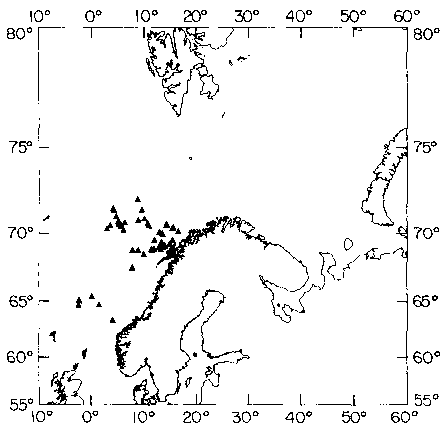
\includegraphics[width = 0.5\textwidth]{figures/whalesitings_large.pdf}
    %\missingfigure{Insert map of LoVe bathymtry here.}
    \caption{Figure from Christensen, 1992.} %\cite{CianoJ.N2001POSW}}
\end{figure}
\end{frame}

\begin{frame}{Bleik Canyon showing 180 documented sightings of sperm whales}
    \begin{figure}
    \centering
    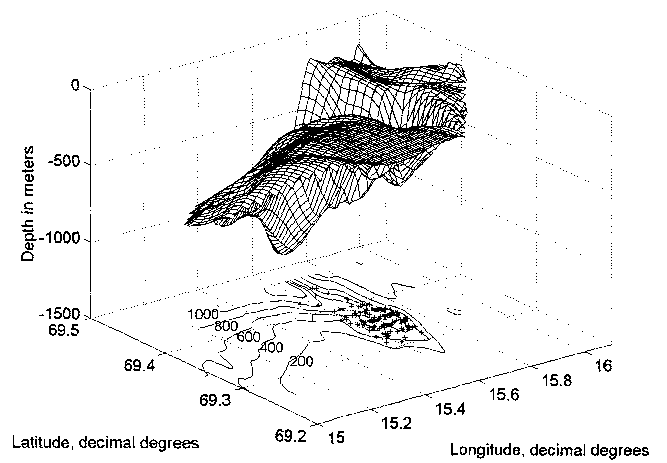
\includegraphics[width = 0.8\textwidth]{figures/whalesitings_bleikdjupet.pdf}
    %\missingfigure{Insert map of LoVe bathymtry here.}
    \caption{Figure from Ciano and Huele, 2001.} %\cite{CianoJ.N2001POSW}}
\end{figure}
\end{frame}

\begin{frame}{The Lofoten-Vesterålen ocean region}
\begin{figure}
    \centering
    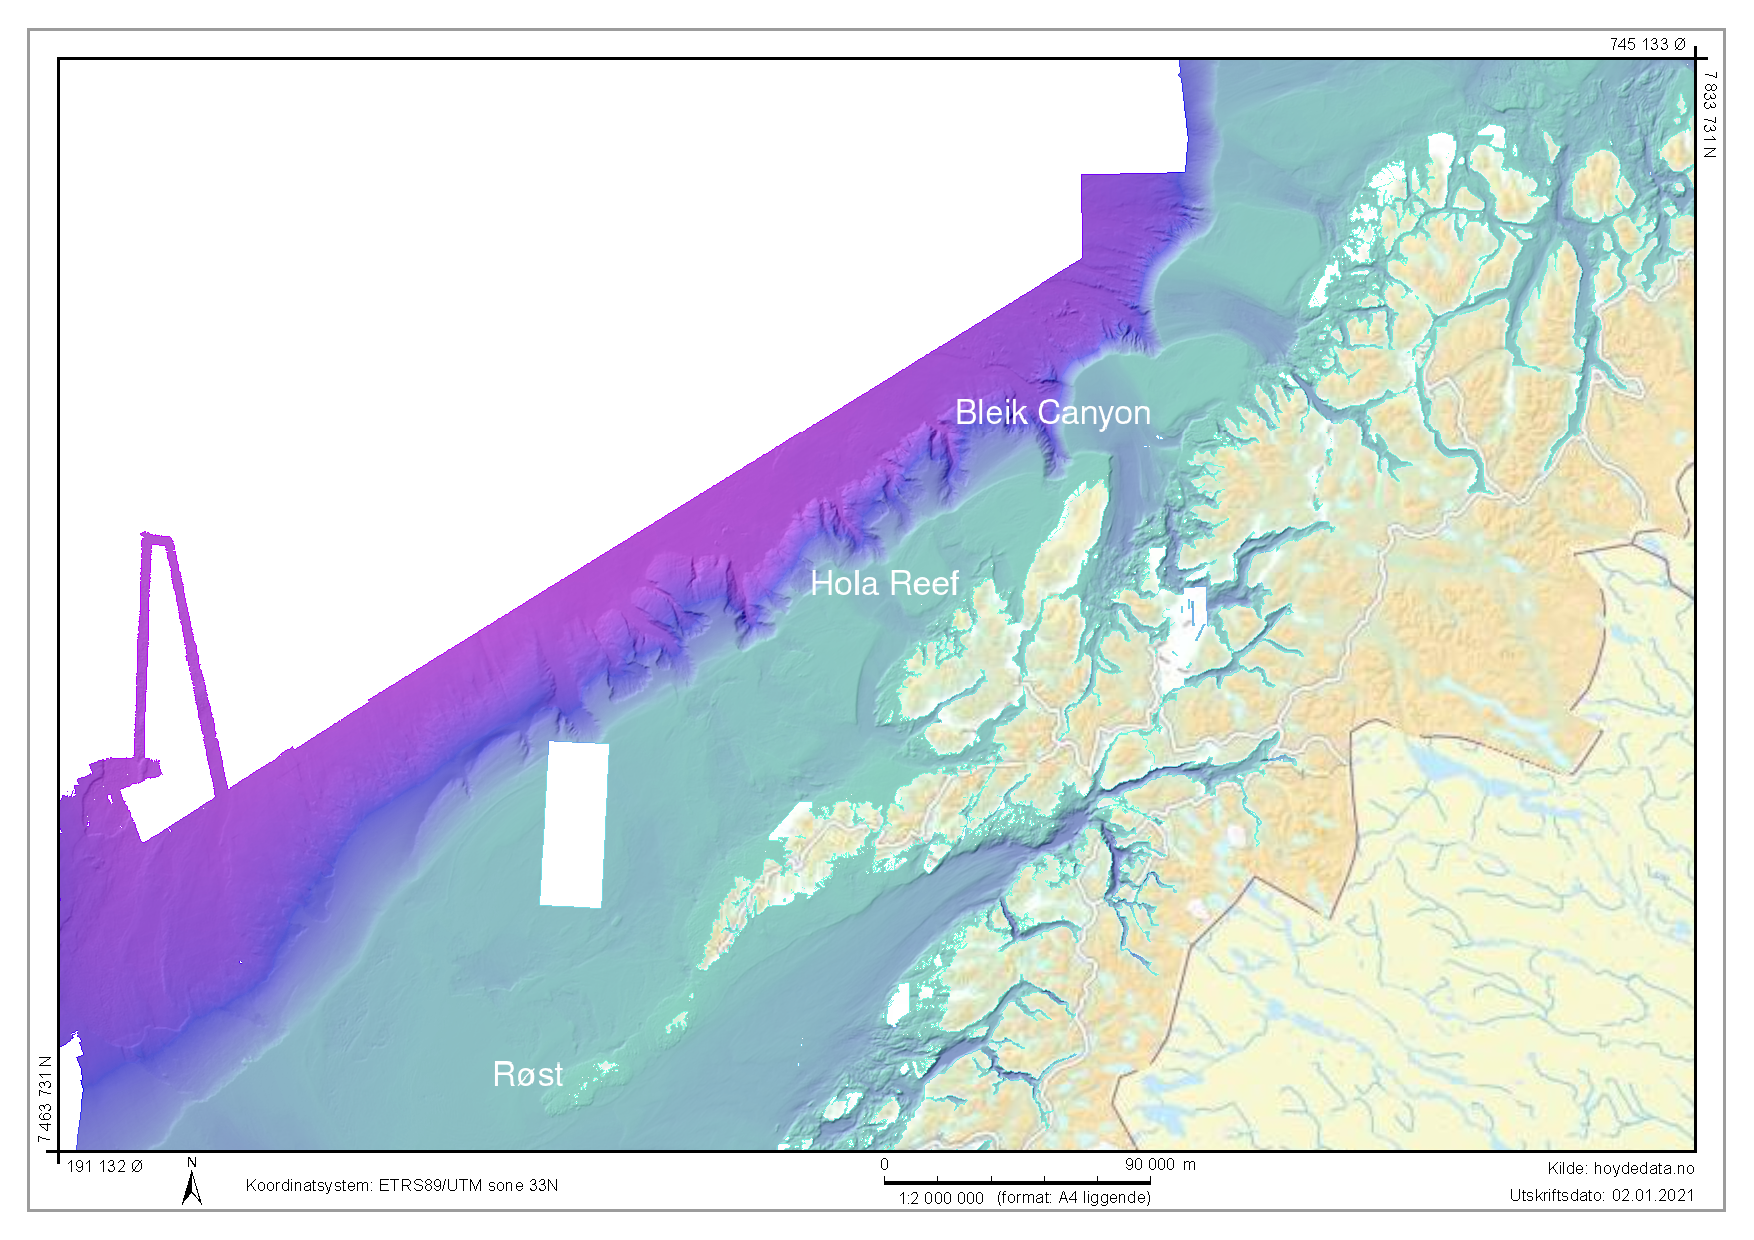
\includegraphics[width=\linewidth]{figures/dybdedata_stor_stedsnavn.pdf}
\end{figure}
\end{frame}

\begin{frame}{Canyon dynamics}
\begin{columns}
\column{0.65\linewidth}
\begin{itemize}
    \item Submarine canyons are steep-sided valleys cut into the seabed of a continental slope.
    \item There is an asymmetrical response to along-shore flow in opposite direction. 
    \item When the flow is retrograde, submarine canyons significantly alter the flow.
    \item Zang and Lentz (2017) suggests this behaviour is due to arrested topographic waves.
\end{itemize}
\column{0.35\linewidth}
\begin{figure}
    \centering
    %\missingfigure{Insert a picture of submarine canyon here.}
    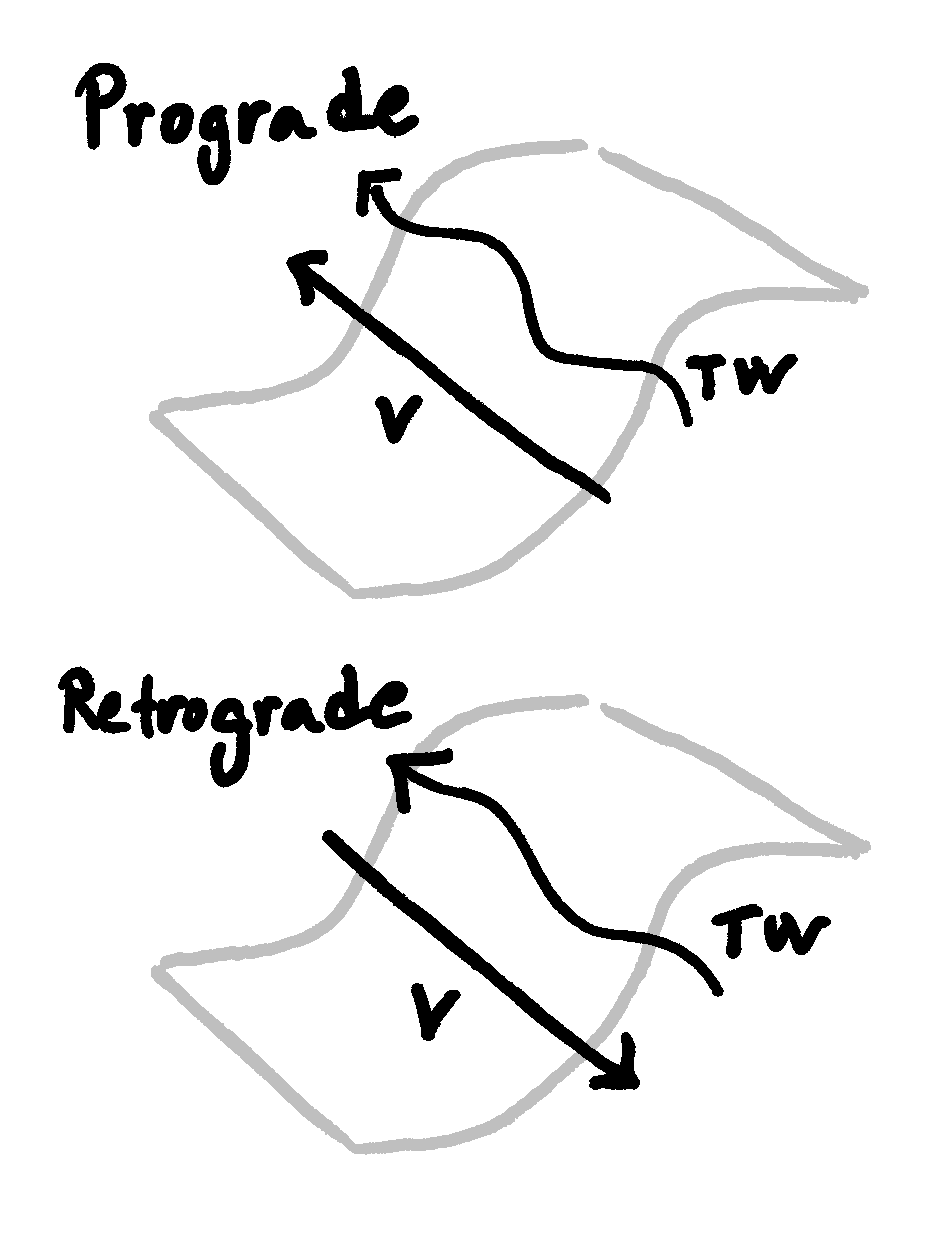
\includegraphics[width=\linewidth]{figures/prograde_retrograde_sketch.pdf}
\end{figure}
\end{columns}
\end{frame}

\subsection{Research questions}

\begin{frame}{Research questions}
    \begin{itemize}
    \item Can quasi-geostrophic theory be used to describe flow patterns over a submarine canyon?
    \item How does high eddy-activity affect the cross-slope exchange due to a submarine canyon?
    \item What is the effect of periods of reversed wind on the cross-slope exchange under mean prograde flow over a canyon? 
\end{itemize}
\end{frame}

\section{Theoretical model}

\begin{frame}{Barotropic flow}
Use the linear barotropic quasi geostrophic vorticity equation. 
Look at a meridional mean flow over a sloping bottom with a canyon: 
\begin{equation*}
    \mathbf{u} = u'\mathbf{i} + \left(V(x)+v'\right)\mathbf{j} \qquad h = \alpha x + h_T(y)
\end{equation*}
Assume a solution on the form
\begin{equation*}
    \psi' = \operatorname{Re}\left[\sum_{k,l,\omega} \hat{\psi}_{k,l}e^{ikx+ily}\right]
\end{equation*}
The Fourier coefficients of the streamfunction response can be written as
\begin{equation*}
    \hat{\psi}_{k,l} = \hat{h}_{k,l}\frac{f_0}{h_0}\left( \kappa^2 + \frac{f_0\alpha}{h_0V} + \frac{\pdd{x}V}{V} - i \frac{r\kappa^2}{Vl}\right)^{-1}
\end{equation*}
Arrested wave number:
\begin{equation*}
    \kappa^2 = -\left(\frac{\alpha f_0}{h_0V} + \frac{\pdd{x}V}{V}\right)
\end{equation*}
\end{frame}

\begin{frame}{Baroclinic flow}
Use the linear baroclinic quasi geostropic vorticity equation. 
Look at a meridional mean flow over a sloping bottom with a canyon: 
\begin{equation*}
    \mathbf{u} = u'\mathbf{i} + \left(V(x)+v'(z)\right)\mathbf{j} \qquad h = \alpha x + h_T(y)
\end{equation*}
%Assume a solution on the form
%\begin{equation*}
%    \psi' = \operatorname{Re}\left[\sum_{k,l,\omega} \hat{\psi}_{k,l}(z)e^{ikx+ily}\right]
%\end{equation*}
The Fourier coefficients of the streamfunction response can be written as
\begin{multline*}\label{eq:baroclinic:sol}
    \hat{\psi}(z) = \hat{h}N\left(\left(\kappa^2 + \frac{\pdd{x}V}{V_0} \right)^{\frac{1}{2}} + \frac{f_0\pd{z}V}{NV_b} + \frac{\alpha N}{V_b} - i\frac{rN\kappa^2}{V_bl}\right)^{-1}e^{-\mu z},\\ \mu = \frac{N}{|f_0|}\left( \kappa^2+\frac{\pdd{x}V_0}{V_0}\right)^{\frac{1}{2}} 
\end{multline*}
Arrested wave number:
\begin{equation*}
    \kappa^2 = \left(-\frac{f_0\pd{z}V}{NV_b} - \frac{\alpha N}{V_b}\right)^2 - \frac{\pdd{x}V}{V_0}
\end{equation*}
\end{frame}

\begin{frame}
\frametitle{Amplitude and phase specters}
\begin{figure}
\centering
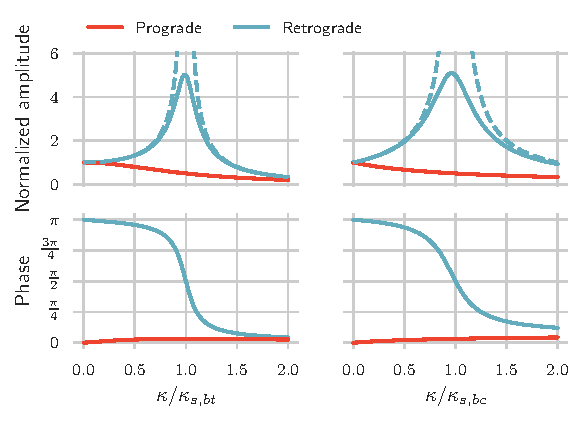
\includegraphics{figures/amplitude_phase.pdf}
\end{figure}
\end{frame}

\section{Numerical experiments}
\begin{frame}
\frametitle{Model bathymetry}
\begin{figure}
\centering
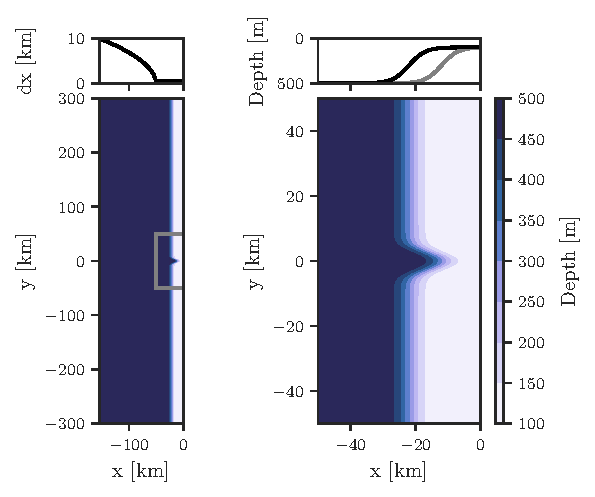
\includegraphics[clip, trim=0 0 0 0.3cm, width=0.8\textwidth]{figures/bathymetry.pdf}
\end{figure}
\end{frame}

\section{Results}

\subsection{General flow pattern}
\begin{frame}
\frametitle{Figure}
\begin{figure}
\centering
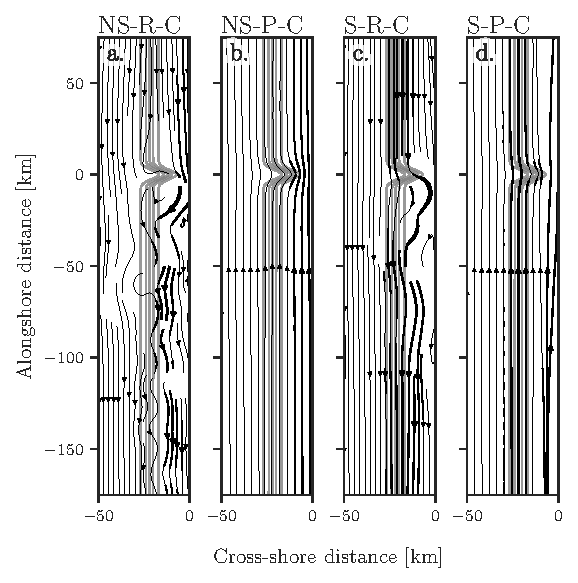
\includegraphics[width=0.7\textwidth]{figures/mean_streamlines_canyon_z95_40-50.pdf}
\end{figure}
\end{frame}

\subsection{Comparison with QG theory}
\begin{frame}
\frametitle{Figure}
\begin{figure}
\centering
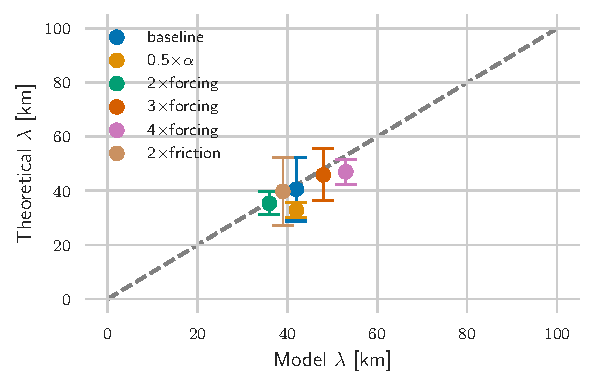
\includegraphics{figures/Unstratified_theoreticalVSmodel_wave_length.pdf}
\end{figure}
\end{frame}

\begin{frame}
\frametitle{Figure}
\begin{figure}
\centering
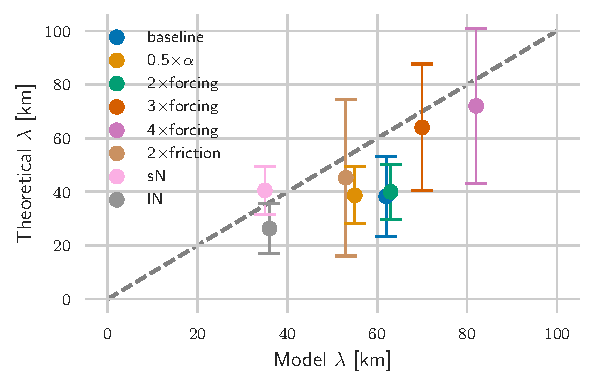
\includegraphics{figures/Stratified_theoreticalVSmodel_wave_length_xzshear.pdf}
\end{figure}
\end{frame}

\subsection{Cross-slope tracer transport}

\section{Discussion}

\section{Conclusion}

\begin{frame}
\frametitle{References}
\footnotesize{
\begin{thebibliography}{99} % Beamer does not support BibTeX so references must be inserted manually as below
\bibitem[Smith, 2012]{p1} John Smith (2012)
\newblock Title of the publication
\newblock \emph{Journal Name} 12(3), 45 -- 678.
\end{thebibliography}
}
\end{frame}

%------------------------------------------------

\begin{frame}
\Huge{\centerline{The End}}
\end{frame}

%----------------------------------------------------------------------------------------
%   SUPPLEMENTARY SLIDES
%----------------------------------------------------------------------------------------
\appendix

\begin{frame}{Supplementary figure}
This slide is not part of total slide count or the navigational panel.
\begin{figure}
    \centering
    \missingfigure{Insert supplementary figure here.}
\end{figure}
\end{frame}

%----------------------------------------------------------------------------------------

\end{document} 